\section{Methods}
The ultimate goal of GateKeeper-GPU is to accelerate the sequence alignment by quickly examining the sequence pairs with fast and accurate pre-alignment filtering, and deciding whether the computationally-expensive alignment is necessary for the genomic sequence pairs. There are four main steps. First, GateKeeper-GPU recognizes system specifications beforehand to allocate memory wisely and enable the extra features accordingly. Using compile-time variables, it calculates every other internal variable during execution via system configuration~(Section 3.1). Second, data buffers are allocated for an optimized data transfer between host and device~(Section 3.2). Third, reads and reference segments are preprocessed for the bitwise algorithm~(Section 3.3) and forth, filtration is applied on each sequence pair by GateKeeper-GPU kernel with an improved GateKeeper algorithm~(Section 3.4). Lastly, we integrate GateKeeper-GPU into mrFAST~\cite{alkan2009personalized} to observe the practical performance gains~(Section 3.5). 

\subsection{System Configuration}
GateKeeper-GPU is designed to require the least amount of user interaction and effort. Because of the disadvantages of dynamic kernel memory allocation of CUDA, read length and error threshold should be specified at compile time. It should be emphasized that the read length variability across different Illumina data sets is low and most of the data sets include 100bp or 150bp reads, therefore the tool recompilation for each dataset is not a frequent necessity.
GateKeeper-GPU starts with configuring the system's properties, such as device compute compatibility since some of the features, like data prefetching, are limited to the compute capability of the system.

Applying the GateKeeper algorithm for a read-reference segment pair is called \textit{filtration}. Since CUDA provides many massively parallel threads, each filtration is performed by a single CUDA thread to have the least possible dependency between the threads for high filtering throughput. Each thread uses the reserved stack frame for the temporary data, such as bitmasks. Before the filtering step, GateKeeper-GPU calculates the approximate memory load of filtration on a thread~(i.e., thread load) using the compilation variables of read length and error threshold. It retrieves the free global memory size of the GPU along with some other GPU parameters, calculates the number of CUDA thread blocks, and the possible number of filtrations for one kernel call~(i.e., batch size) to fully utilize GPU for boosting performance. Since data transfers between the device and host are expensive, the configuration step ensures that the batch size is maximized to keep the total number of transfers minimal. In the multi-GPU model, the batch size is equal for all devices to ensure a fair workload. In this way, we adjust the kernel parameters of efficient GPU usage for the device model and memory status without the user’s concern.

\subsection{Resource Allocation}
The main algorithm consists of simple bitwise operations. Distributing the workload of one filtration between multiple threads would introduce overheads emerging from inter-thread dependencies rather than speeding up the process. Therefore, each thread runs kernel function for a single filtration with the least dependency possible. 

GateKeeper produces \textit{2e + 1} Hamming masks to store the intermediate bitvectors for indels~(i.e., insertions and deletions) where \textit{e} is the error threshold. Since CUDA dynamic memory allocation inside device functions is restricted and slow, we use fixed-size unsigned integer arrays for bitmasks in the kernel. For this reason, GateKeeper-GPU requires read length and error threshold at compile time. Each thread uses the reserved stack frame in thread-local memory for bitmasks, which is cached in unified L1/Texture and L2 cache for Pascal architecture; in L1 and L2 cache for Kepler architecture~\cite{programmingGuide}. All of the constant variables and the look-up table~(LUT) for the amending procedure are stored in the constant memory.

We utilize unified memory for the read buffer and the reference for providing simplicity and on-demand data locality. As the number of filtration operations per batch is determined in the system configuration stage, a read buffer is created in unified memory together with candidate reference indices corresponding to the reads. Since the number of candidate reference locations is unknown until seeding, batch size does not limit candidate reference location count, thus there is no predefined value of reference segment count per read.     

\subsection{Preprocessing}
Once the system properties are recognized and parameters are adjusted accordingly, GateKeeper-GPU starts to prepare the reads and the reference for filtration. The main portion of preprocessing involves encoding the strings to 2-bit representations for bitwise operations. Since each character takes up two bits after encoding, a 16-character window is encoded into an unsigned integer (i.e., one word), thus a 100bp read is represented as seven words in the system.    

GateKeeper is designed for DNA strings, hence it only recognizes the characters \textit{`A', `C', `G'} and \textit{`T'}. Occasionally, the reads or the reference may contain the character \textit{`N'} that signals for an unknown base call at that specific location of the sequence. Because GateKeeper does not recognize the character \textit{`N'}, GateKeeper-GPU directly passes those sequence pairs from the filter without applying filtration steps as a design choice for two reasons: first, supporting an extra character requires expanding the encoding to 3-bit representations which unnecessarily increases the complexity and memory footprint for this rare occasion; second, since these unknown bases add extra uncertainty, leaving the decision to verification increases credibility. 

Assigning the encoding job to either the host~(i.e., CPU) or the device~(i.e., GPU) creates advantages and disadvantages from different perspectives. Encoding in the host and copying the encoded strings to the device is cost-effective in data transfer since encoding compresses the strings into smaller units. However, processing in the host can be stagnant even if it is multi-threaded compared to massively parallel processing in the device. Conversely, allowing each device to encode the strings for their own operations adds extra parallelism to the whole execution while reducing the efficiency in transfer time. We provide GateKeeper-GPU in both versions and analyze the effect of the processor in encoding on overall performance, which will be discussed further in the Evaluation section.

In most of the read mappers' workflow, first, the possible reference locations are found, the read is verified, and then the same operations are carried out for the next read. Multi-threaded mappers allow the processing of several reads at a time. Nevertheless, it is necessary to utilize the maximum number of threads possible per kernel call for an effective GateKeeper-GPU execution by fully employing the GPU resources. Therefore, many read and their candidate reference segments are prepared and batched in the host for a single kernel before verification, depending on the pre-calculated batch size.

\subsection{GateKeeper-GPU Kernel}
When the buffers are ready for execution, we set the usage patterns of the buffers in terms of caller frequency about the host or the device by CUDA memory advice API. Since the kernel utilizes the buffers more than CPU functions until the next batch of reads is processed, the preferred location of the data is set to be the GPU device for the input buffers for the kernel. According to the assigned memory advice for each buffer, the data arrays are prefetched asynchronously ahead of the kernel function to provide an early start for data migration from host to device, and mapping data to the device's page tables before kernel accesses~\cite{programmingGuide}. Since there is more than one buffer for prefetching, each buffer is asynchronously submitted to a different stream. Memory advice mechanism and prefetching are supported for compute capability $6.x$ and later, therefore these actions are skipped for lower CUDA compute capabilities.

After prefetching, the kernel function is executed with the parameters for the number of blocks and threads that are previously set in the configuration stage. The kernel performs the complete set of operations for a single filtration, starting with encoding the sequences if they are not encoded in the preprocessing stage. 

Due to architectural differences between FPGA and GPU, some alterations are applied to maintain the GateKeeper algorithm in C-derived device functions in GPU. In contrast to FPGA's specialty in bitwise operations, GPU does not support bitvectors in arbitrary sizes. An encoded 100bp read can be represented as a 200-bit long register in FPGA, whereas GPU allocations are limited with the word size of the system, thus the encoded read becomes an array of 7 words. Additionally, logical shift operations produce incorrect bits between array's elements. For correcting these bits, we apply \textit{carry-bit} transfers. The correction procedure must be performed for each bitwise shift, such that there are \textit{2e} shifts and \textit{2e} carry-bit operations~(insertion and deletion masks each require \textit{e} operations) in the filtration with an error threshold of \textit{e}. 

Bitwise shift operations leave the most significant or the least significant bits vacant, depending on and opposite to the shift direction. Even though these bits should be $1s$ on the final bitvector signaling for errors, the final AND operation on all masks hide these errors since the corresponding bits are $0$ in the shifted masks. MAGNET~\cite{alser2017magnet} previously addressed this issue by solving it with a combination of steps. In order to uncover these possible errors on leading and trailing parts, we add a single OR operation to turn the excess bits into $1s$ after preparing amended masks. In this way, we ensure that the leading and trailing bits are $1$ even if the XOR operation for the Hamming mask converts them into $0$. Figure \ref{fig:imp_mini} shows how the new amended mask covers the leading and trailing $0$, which is missed by GateKeeper~\cite{Alser2017}. 
\vspace{-2mm}
%%%%%%%%%%%%%%%%%%%%%%%%%%%%%%%%%%%%%%%%%%%%%%%%%
% Fig: improvement in alg. mini fig
\begin{figure}[!htbp]
\centering
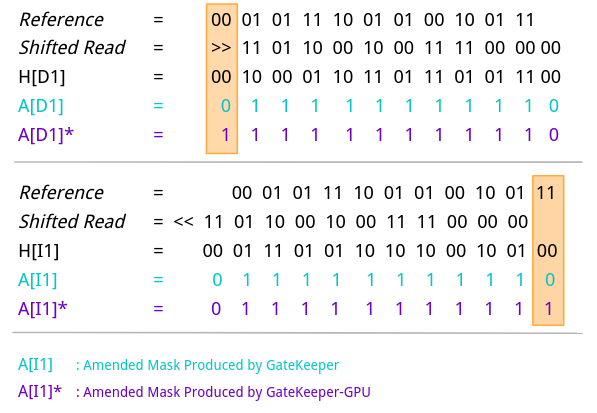
\includegraphics[width=0.35\textwidth]{figures/imp_mini.png}
\caption{Strategy for improving leading and trailing 0 bits. \textit{Reference} and \textit{Shifted Read} show bitvectors of candidate reference segment and shifted read, respectively; \textit{H} and \textit{A} represent Hamming mask and amended mask.}
\label{fig:imp_mini}
\begin{minipage}{0.49\textwidth}
\vspace*{0.1cm}
\end{minipage}
\end{figure}
%%%%%%%%%%%%%%%%%%%%%%%%%%%%%%%%%%%%%%%%%%%%%%%%%%%

As a result of this modification, GateKeeper-GPU can reject some of the read and reference segment pairs that exceed the error threshold, which GateKeeper falsely accepts. Figure \ref{fig:imp_big} shows the amended masks produced by GateKeeper and GateKeeper-GPU for the same sequence pair for error threshold \textit{e} = 2. This improvement enables GateKeeper-GPU to make the correct decision for rejecting the pair, whereas GateKeeper falsely accepts the pair.
%%%%%%%%%%%%%%%%%%%%%%%%%%%%%%%%%%%%%%%%%%%%%%%%%
% Fig: improvement in alg. imp big
\begin{figure}[!htbp]
\centering
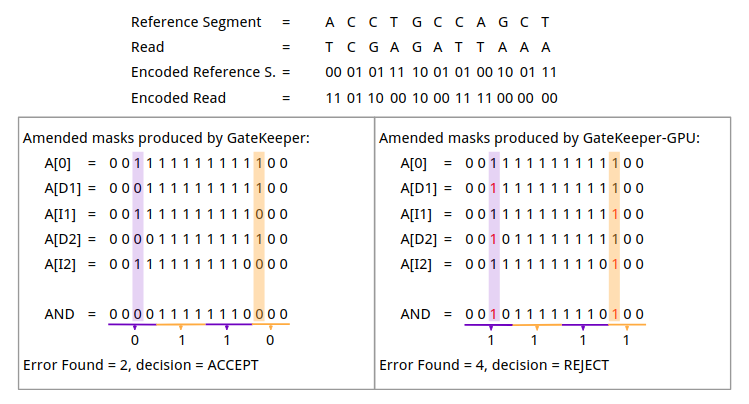
\includegraphics[width=0.5\textwidth]{figures/imp_big.png}
\caption{Amended masks produced by GateKeeper \cite{Alser2017} and GateKeeper-GPU.}
\label{fig:imp_big}
\end{figure}
%%%%%%%%%%%%%%%%%%%%%%%%%%%%%%%%%%%%%%%%%%%%%%%%%%%

It should be emphasized that GateKeeper-GPU does not perform seeding, and it is not a kmer filter. It relies on the candidate reference locations reported by the mapper and performs filtration only on the read and reference segment pairs, which are expected to match with the mapper's high confidence. Further, GateKeeper-GPU does not calculate but \textit{approximates} the edit distance between pairs for fast filtration. The verification performs the exact edit distance calculation, and GateKeeper-GPU acts as an intermediate step in preparation for verification.

\subsection{Adaptation to mrFAST Workflow}
We integrate GateKeeper-GPU into mrFAST to evaluate its performance on the whole genome scale, as briefly illustrated in Sup. Figure S.2. GateKeeper-GPU can be adapted to any short read mapping tool that uses seed extension, and in this section, we present the necessary adjustments. We begin with encoding and loading the reference into the unified memory using multithreading with OpenMP. While encoding, the locations of \textit{`N'} bases on the reference genome are also recorded since the segments containing this character will not be evaluated in the filtering stage. 

In the original workflow of mrFAST, candidate locations of a single read are found and verified, mapping information of the read is recorded, then the next read is processed. Since GateKeeper-GPU requires batching, we fill the buffers with multiple reads and their candidate location indices with partial multicore support. The number of candidate locations of a particular read cannot be anticipated before seeding, therefore there are two factors that dynamically control the size of buffers to ensure that GPU utilization is optimized without exhausting the resources: the number of filtration pairs that is calculated by the system configuration unit~(Section 3.1) and the number of reads allowed per batch. The number of reads is predetermined and in our experience with different values~(Table \ref{tab:maxnumreads}), we find that $100,000$ reads yield the best results for mrFAST. We observe that using $100,000$ reads per batch decreases the overall runtime, durations of the kernel, and filter since the number of transfers between the host and the device is minimized. Still, the maximum number of reads is a parameter for execution and can be modified easily according to the desired mapper or execution.

%%%%%%%%%%%%%%%%%%%%%%%%%%%%%%%%%%%%%%%%%%%
% table: Max num read per batch vs time
\begin{table}[!htbp]
\caption{Effect of the maximum number of reads processed per batch on time~(seconds).}
\label{tab:maxnumreads}
\begin{adjustbox}{max width=0.49\textwidth}
\Large
\begin{tabular}{r|rrrr|rrrr}
\multicolumn{1}{c}{}                          & \multicolumn{4}{c}{\textbf{Encoding in Host}}                                                                                                            & \multicolumn{4}{c}{\textbf{Encoding in Device} }                                                                                                           \\
\multicolumn{1}{c|}{ \textit{Max. \# Reads} } & \multicolumn{1}{c}{\textit{Overall} } & \multicolumn{1}{c}{\textit{Encode }} & \multicolumn{1}{c}{\textit{Kernel }} & \multicolumn{1}{c|}{\textit{Filter} } & \multicolumn{1}{c}{\textit{Overall} } & \multicolumn{1}{c}{\textit{Copy} } & \multicolumn{1}{c}{\textit{Kernel }} & \multicolumn{1}{c}{\textit{Filter} }  \\ 
\hline \rule{0pt}{2ex}
100                                           & 3,041.52                              & 109.54                               & 102.55                               & 212.17                                & 2,944.59                              & 100.19                             & 105.39                               & 187.58                                \\
1000                                          & 1,446.58                              & 105.99                               & 92.72                                & 114.61                                & 1,335.20                              & 77.55                              & 97.20                                & 116.29                                \\
10,000                                        & 1,325.95                              & 109.14                               & 80.37                                & 92.99                                 & 1,322.96                              & 84.45                              & 83.22                                & 92.29                                 \\
100,000                                       & 1,275.66                              & 103.13                               & 77.45                                & 88.96                                 & 1,215.25                              & 75.19                              & 82.37                                & 91.17                                \\
\hline 
\end{tabular}
\end{adjustbox}
\begin{minipage}{0.49\textwidth}
\vspace*{0.2cm}
{\scriptsize
These measurements were recorded during the mapping of Chromosome 1. Kernel: Total filtering time measured by CUDA API, Filter: Total filtering time measured from the host side.}
\end{minipage}
\end{table}

%%%%%%%%%%%%%%%%%%%%%%%%%%%%%%%%%%%%%%%%%%%%%

Once the data transfer buffers are filled, the kernel function is called with the previously calculated number of blocks and threads parameters. Each thread executes a single comparison, starting with extracting the relevant reference segment based on the index. The result of the filtering decision as `1'~(\textit{accept}) or `0'~(\textit{reject}), and the approximated edit distance are written back on the result buffers in the unified memory. 

The only synchronization point for threads is after the completion of the filtering step for one batch. Since the host and device use a common pointer for buffers in the unified memory model, the threads' job needs to be completed in order for verification to obtain filtering results. The pairs that pass the filter are verified, and mrFAST continues with further steps to report the mapping information.